\section{Limiter}
Instead of equalizing the signal it is possible to limit the signal instead by using a limiter. A limiter limits the signal at a certain threshold to make sure that a signal does not clip or that a membrane does not hits its coil. A limiter system is a feedforward system which can be stated as:
\begin{equation}
y(n) = g(n)\cdot x(x-D)
\end{equation}

Where an input $x(n)$ is delayed by $D$ and multiplied by a weigthing $g(n)$ to give $y(n)$, or as a logarithmic level representation where multiplication leads to the addition of $G_{dB}(n)$ and $X_{dB}(n)$:
\begin{equation}
Y_{dB}(n) = X_{dB}(n) + G_{dB}(n)
\end{equation}

A limiter system is also seen in more detail on \autoref{fig:limiter_block}.

\begin{figure}[H]
\centering
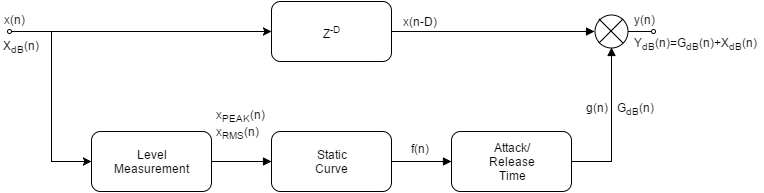
\includegraphics[width=1\textwidth]{figures/Limiter_block.png}
\caption{Limiter block diagram.}
\label{fig:limiter_block}
\end{figure}   

\todo[inline]{referencen Digital_Audio_Signal_Processing bogen kapitel 7}

The level measurement block measures the RMS or peak value of the signal, the static curve applies the gain and the Attack/Release time determines when the limiter should apply and stop applying to the signal. The static curve more detailed described the curve which determines at which the noise gate threshold (NT), expander threshold (ET), compressor threshold (CT) and limiter threshold (LT) should apply as seen on \autoref{fig:limiter_static}. 

When these different thresholds are surpassed a specific linear function will be applied to the signal to for example filter out noise (NT) or compress the signal to limit the output relative to the input as seen on \ref{fig:limiter_static}. 

\begin{figure}[H]
\centering
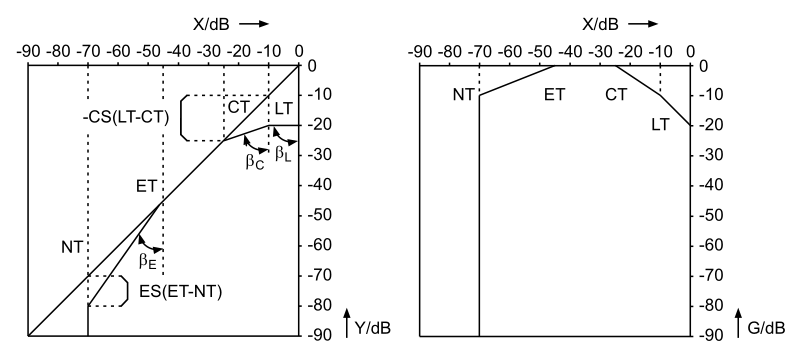
\includegraphics[width=0.8\textwidth]{figures/limiter_static_curve.png}
\caption{Static curve with the parameters (LT, CT, ET and NT).}
\label{fig:limiter_static}
\end{figure}  

Because the focus will be on limiting the signal and not clipping it, which would introduce to much distortion, the focus should be on CT which compresses the signal. The compressor can be designed for hard compression which limits the output more than a soft compression but it also creates more distorted output. The compressor can either apply to all frequencies or be a multiband compressor which only applies to the frequency spectrum which needs compression, which gives a more flexible compressor but also increases the complexity of the system.    

      